\chapter{The IceCube Experiment}

hier tot pg 75?

Ook de voornaamste zoektochten van IceCube vermelden en duiden. Bv de point sources, astrophysical (Sam zijn thesis bv) etc.


Iets van wavelength dependence van Frank-Tamm:

\begin{equation}
\frac{dN}{dx} = \int_{\lambda_1}^{lambda_2} \frac{2 \pi \alpha}{\lambda^2} \sin^2 \left(\theta_c\right) d\lambda = 2\pi \alpha \sin^2 \left(\theta_c\right) \left(\frac{1}{\lambda_1} \frac{1}{\lambda_2}\right).
\end{equation}

Copy paste van Wikipedia:
 Data from the Fermi Space Telescope (2013)[3] have been interpreted as evidence that a significant fraction of primary cosmic rays originate from the supernova explosions of stars.[4] Active galactic nuclei also appear to produce cosmic rays, based on observations of a neutrino and gamma rays from blazar TXS 0506+056 in 2018.[5][6]
 

\subsection{Muon tracks}
Ook muonen van atmosfeer, in hfdstk 4 enkel over muonen van neutrinos gebabbeld.
intro intro
The track-like structure of the signal allows to find a good ``lever arm'' as the deposited charge on the earliest and latest DOMs provide strong constraints on the event's position, time and direction. As a result, directional reconstruction..... Muons can transit the entire detector, making it difficult to reconstruct the energy of the muon and the parent neutrino. Starting muon tracks are challenging, but more useful to infer the initial energy of the neutrino. Highly relativistic muons are stochastic in nature and the energy loss depends on the energy of the particle. Using equation ??? it is possible to have a better energy reconstruction.
\subsection{Cascades}
The light output has a slight asymmetry in the direction of motion, making directional reconstructions challenging. However, these interactions are often calorimetric and therefore allow for nearly complete measurements of the energy and result in a good energy resolution.

\begin{figure}
\label{fig:ICinteractions}
\centering
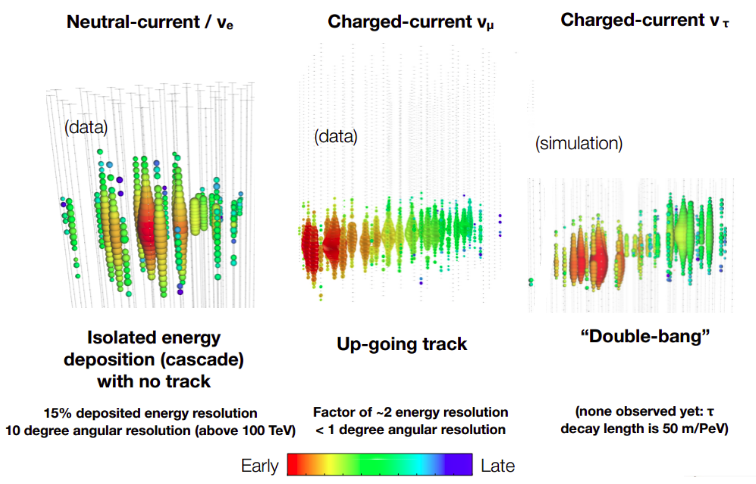
\includegraphics[width=\textwidth]{chapter4/img/ICinteractions2.png}
\caption{Neutrino interactions in the IceCube detector have two distinct types of interactions: cascades and tracks. Energetic taus are theorized to have double-bang signatures but have not undeniably been seen. Colors determine the timing of hits in the optical modules in the ice. Illustrations from the IceCube collaboration.}
\end{figure}